% Going off the Thesis guidelines available here: http://www.lboro.ac.uk/students/welcome/research/codes-of-practice/appendices/
% A4 paper size selected, default is 11pt font, to change to 12pt use [a4paper, 12pt] as option to documentclass
\documentclass[a4paper]{report}

% Some useful packages for including images, colored font, etc.
\usepackage[dvips]{graphicx}
\usepackage{listings}
\usepackage{url}
\usepackage[pdftex,dvipsnames]{xcolor}
\usepackage{graphicx}
\usepackage{pgfgantt}
\usepackage{float}
\usepackage{fancyvrb}

%Bibliography Setup
\usepackage{natbib}
\bibliographystyle{agsm}

% Set margins in all document to 3.5cm as per guidelines for binding
\usepackage[includeheadfoot,margin=3.5cm]{geometry}

% Used to including pdf files within pages
% use [draft] as option to output empty spaces rather than rendering all pages (useful when including lots of pdfs)
\usepackage{pdfpages}

% Used to produce headers and footers
\usepackage{fancyhdr}
\pagestyle{fancyplain}

% Used for removing title in bibliography sections
\usepackage{titlesec}

%Todo commands
\usepackage{xargs}
\usepackage[colorinlistoftodos,prependcaption,textsize=tiny]{todonotes}
\newcommandx{\unsure}[2][1=]{\todo[linecolor=red,backgroundcolor=red!25,bordercolor=red,#1]{#2}}
\newcommandx{\change}[2][1=]{\todo[linecolor=blue,backgroundcolor=blue!25,bordercolor=blue,#1]{#2}}
\newcommandx{\info}[2][1=]{\todo[linecolor=OliveGreen,backgroundcolor=OliveGreen!25,bordercolor=OliveGreen,#1]{#2}}
\newcommandx{\improvement}[2][1=]{\todo[linecolor=Plum,backgroundcolor=Plum!25,bordercolor=Plum,#1]{#2}}
\newcommandx{\thiswillnotshow}[2][1=]{\todo[disable,#1]{#2}}

% To have a separate bibliography per Chapter uncomment this line

% See Introduction/Introduction.tex for example how to include the bibliography
%\usepackage{chapterbib}

% Line spacing defined at 1 and a half. I know it says 1.3 but its 1 and a half.
\linespread{1.3}

% Setup headers and footers
\fancyhf{}
\lhead{\leftmark}
% Page number placed on right side on odd pages and left side on even pages
\fancyfoot[RO, LE] {\thepage}

\begin{document}

% Give \subsubsection numbers
\setcounter{secnumdepth}{4}

% Title, Author, Abstract, Acknowledgement, Table of Content, List of Figures and List of Tables
% !TeX root = ../main.tex

% Front content of the Dissertation
\title{Secure Smart Lock System}

\author{by\\Zack Pollard\\
\\
{\bf A Final Year Dissertation}\\
\\
Submitted in partial fulfilment of the requirements for the award of\\
BSc Computer Science of Loughborough University\\
\\
\copyright
\hspace{1 dd} Zack Pollard 2018\\
\\
April 2018
}
\date{} % Used to remove date from title so it can be set at any date rather than the current date

\maketitle

% Set page numbers to roman numerals for front matter
\pagenumbering{roman}

% PDF exports of Word Documents available (Exported August 2012)
% Thesis Access Form
%\includepdf[pages=1, pagecommand=, templatesize={5in}{10in}]{Front/LU/access.pdf}
% Certificate of Originality
%\includepdf[pages=-, pagecommand=, templatesize={5in}{10in}]{Front/LU/origin.pdf}

% Abstract
\chapter*{Abstract}
\addcontentsline{toc}{chapter}{Abstract}
%Include an abstract of your Thesis, should be around 300 words (1 side of A4).
%The abstract immediately follows the title page, and is presented on a page on its own.
%It consists of a brief summary of no more than 300 words which accurately outlines the
%main aims and achievements of your dissertation.


% Acknowledgements
\chapter*{Acknowledgements}
\addcontentsline{toc}{chapter}{Acknowledgements}
%In this section you should acknowledge those who have helped you or offered you advice
%during your project. It is common courtesy to include an acknowledgement to
%your project supervisor. People sometimes also include acknowledgement of family and
%friends who have helped to proof-read the work or provided emotional support. The
%acknowledgement should be brief and succinct.

% Set the depth for your table of content
% Currently set at 2 (Chapter, Section, Subsection)
\setcounter{tocdepth}{2}
% Include a table of content
\tableofcontents
%This section should be be entitled “Contents” and should provide a list of chapter,
%section and subsection headings with their appropriate page number. You are strongly
%advised to use the features provided within LATEX or your word-processing software to
%auto-generate this page. This ensures that the details are correct and reduces a lot of
%labour-intensive and painstaking work. An example contents page is provided at the
%start of this document (although you should note that this document is in ‘article’ style
%and therefore not structured with chapters as a dissertation would be).

% Include a list of figures
\listoffigures
\addcontentsline{toc}{chapter}{List of Figures}

% Include a list of tables
\listoftables
\addcontentsline{toc}{chapter}{List of Tables}

\newpage

% Set page numbering to arabic for body of Thesis
\pagenumbering{arabic}

% Introduction
%This section will be relatively short. It should introduce the reader to the problem that
%is to be tackled, and provide a brief indication of the context within which the problem
%exists. This will include some consideration of appropriate related literature and/or
%past attempts at solving the problem, although the main consideration of previous work
%should be left until the Literature Survey. The most important part of the introduction
%is the identification of why the problem is of particular interest and worthy of further
%study. The introduction should seek to draw the reader into the remainder of the
%dissertation, whetting their appetite to learn more of the problem and its solution. It
%should introduce the structure of the document and provide a framework for the reader
%as progress is made through the remainder of the dissertation.
\chapter{Introduction}
\label{chap:intro}
\info{Zack, you need to explicitly tell the novelty of your project in this opening chapter. You have made some high-level statements such as ``...to create a product unlike these other smart home devices...'', but you need to make technical arguments too.}

\section{Problem Statement}
\info{be more specific on the weaknesses of August and how your project will differ/improve these}
With smart devices being created left right and centre nowadays with very little care towards security, it is going to become more common that houses are being hacked with devices slowly controlling more and more sensitive areas of the home. An example of this would be the August lock, an idea similar to what I am trying to achieve here, however the device has multiple security flaws that were found and outlined at the security conference Defcon\info{references and examples}. This is far from the first smart home device that was found to have security issues, there have been hundreds of different WiFi Security cameras that connect themselves to the web with little care towards the security of that device which has the capability of letting someone spy on your home. Not to long ago, there was a huge attack that brought down DynDNS, and therefore all the sites that used it which included Twitter, Spotify and Reddit. \info{references} This attack was using the internet connections of innocent people who happened to have insecure smart home devices in their homes. Millions of smart home devices were involved in the attack as they were hacked due to their inadequate or sometimes non-existent security.
\newline
\newline
The proposed solution was to create a product unlike these other smart home devices, one that is secure enough that I would be happy to put it in my own home. At the end of the day, a camera being infected doesn't matter so much, but a system that unlocks your house needs to be bulletproof on the security front. Looking at the implementation of the August lock, it just isn't something that I would be willing to use to secure my house, yet thousands, maybe more unknowing customers have purchased the august lock and use it to secure their homes every day. I want to create something that is easy to use and secure, something that most companies seem to have trouble with nowadays.

\section{Aims and Objectives}

\subsection{Aim of the Project - Technical}
The project objective is to create a smart lock system that would be able to automate the unlocking and locking of a house's front door. The system will be comprised of multiple Raspberry Pi's with sensors connected to them to retrieve data from a variety of sources to determine whether the door should be locked or unlocked. The system will use RESTful APIs so that it can be easily extended to more devices in the future, and will ensure that all communication between devices is done so in a fully encrypted and secure manner. An example of some authentication methods that the system may use would be fingerprint, RFID/NFC, Facial Recognition, etc.
\newline
\newline
Security is key as this will be securing a home. It is imperative that all communication is done securely, and that the system is certain that the user is who they say they are before they let them into the house. I will be conducting research into the best and most accessible security methods that could be used for this project for the initial implementation and demonstration. The idea however, is that the system will be built in such a way that anyone could create a device for this system using the RESTful APIs that will be available from the core control centre in the house.

\subsection{Aim of the Project - For the User}
So security is all well and good, but the product must still be easy to use for the user. At the end of the day, a lot of users don't care about how secure a product is, and will trust that the company has put in the correct security measures. This reason alone is why there are so many unsecured smart devices out in the wild as your average person doesn't have the technical knowledge to ensure that the product is secure. The companies that make these products know this and so don't actually implement robust security, something that, in my opinion, should be regulated more closely. This product should make the users lives easier whilst still maintaining the security of any normal key based locking system.
\newline
\newline
A simple run down of what I would want from this lock for the user would be the following. They walk up to their home after having setup their system, and all they need to do to get in is tap their phone on the NFC pad in order to unlock the door, and have it lock itself again after they have entered the house, probably on a timer of some sorts. If the door fails to lock for any reason, the user should be notified (another issue with the august lock, if it fails to lock, it simply reports the door as locked, even if it isn't).

\subsection{Project Objectives}
\begin{itemize}
	\item Design a Database Schema that can be used to store all the users data and settings efficiently \info{how can you measure this?}
	\item Develop a core application for the house that will control the main system functions
	\item Develop a REST API for the core application that other systems (i.e. authentication systems) can talk to
	\item Implement a minimum of two authentication methods that can be used to unlock the door
	\item Develop a server system that can be used for the core to sync with and for the user to communicate with the system when outside of the home
	\item Develop a minimal Android application that the user can use to setup and manage their system
	\item Ensure that the security of the product is solid and that all communication is secured with TLS 1.2
\end{itemize}


%\section{Problem Formulation}
%
%\section{Aims and Objectives}
%
%\section{Outline of Areas of Research}
%
%\subsection{Sub Section 1}
%
%\subsection{Sub Section 2}
%
%\subsubsection{Sub Sub Section 1}
%
%\subsubsection{Sub Sub Section 2}
%
%\subsubsection{Sub Sub Section 3}
%
%\subsubsection{Sub Sub Section 4}
%
%\subsection{Sub Section 3}
%
%\section{Contribution of Thesis}
%
%\section{Thesis Outline}

% Literature Review
% !TeX root = ../../main.tex
\chapter{Literature Review}
\label{chap:literature_review}

\section{Aim}
Investigate different aspects of a secure smart lock system to see where potential security issues could be and how to avoid or counteract them.
\section{Objectives}
\begin{itemize}
	\item {Evaluate different areas of the Secure Smart Lock System}
	\item Investigate methods of ensuring the security of the system
	\item Investigate ways to avoid potential security risks imposed by necessary parts of the system
	\item Ensure that security doesn't make the system considerably more difficult for the user to setup, use day-to-day or manage
\end{itemize}

\section{Current Smart Locks}
Smarts locks and internet of things (IoT) devices, in general, have increased massively in availability and use over the last couple of years and according to \cite{Buhov2016}, there will be 50 billion devices connected to the internet by 2020. Having these devices in and around your home constantly connected to the internet introduces some risk if they are not properly secured. This risk is exaggerated if they are devices that secure your home such as a smart lock.
\\
\indent\cite{Ho2016} compare 5 commonly available smart locks that are on the market right now. These locks operated in three different ways: touch-to-unlock, mobile app unlocking, and automatic unlocking. For my purposes, I am mostly interested in the mobile app unlocking as it will be the main way to unlock the Secure Smart Lock System. All the smart locks except for the Lockitron connect to the internet through a Bluetooth connection to the phone, rather than connecting directly, this is interesting as my system will only use Wi-Fi, and will only communicate directly with the phone if they are on the same Wi-Fi network.  The study concluded that all the smart locks except for the Lockitron were vulnerable to the attacks that they undertook, this was down to the Lockitron using Wi-Fi directly and therefore being able to verify with the server for the most up-to-date access control lists. They continue to explain that direct connections, while good, do mean that the device must include a Wi-Fi module which increases power usage on the device and so battery-only operation isn't feasible. A good point they make about the Lockitron is that it doesn't maintain its own access control list locally, so in the event of their servers being unavailable, the lock will not function. This is something I plan to avoid in my lock by maintaining a local access control list, however, due to the attacks mentioned in the study, I will ensure that any changes to the access control list are passed onto the lock before the user is told they are saved.
\\
\indent\cite{Ye2017} did a study specifically on the security of the August Smart Lock. This study focussed on more specific attacks such as moving the owner account from one phone to another and taking control of it. All of the attacks that they performed required root access to the Android device in order to perform, which is unreasonable to assume you will be able to get without taking the users device and knowing their unlock code to perform the rooting process. This is further shown by \cite{Fuller2017} who also tried to penetrate the August Lock but without using rooting as their main point of entry. The attacks that \cite{Ye2017} performed certainly aren't ideal, but rooting compromises the integrity of the device and exposes all the data on the device including encryption keys, app data and anything else the device has stored. As shown by \cite{Fuller2017} the August Lock has had a lot of past security issues, however, they have been fixed by the development team since then.

\section{Certificate Pinning}
Certificate pinning is one of many ways to ensure you are talking to the server you think you are. If you end up doing this badly, however, you can decrease the security of your app. A study performed by \cite{Buhov2016} does an evaluation of 25,000 android apps on the play store to see how many of them implement security properly. It turns out that only 21\% of applications have no issues, with 36\% having a broken implementation of either the Trust Manager or the Hostname Verifier. This issue is brought about by people using self-signed certificates or pinning certificates and trying to, therefore, implement their own version of the Trust Manager and/or Hostname Verifier but doing so incorrectly. As pointed out by the study, many of the incorrect implementations of the Trust Manager lead to the app accepting any certificate it was given, therefore breaking the chain of trust that is usually in place on the device. \cite{Tendulkar2014} back this up showing that out of the apps they tested, only 43\% use SSL verification correctly with the remaining apps either accept all certificates or accept all hostnames. An even more interesting fact that they discovered was that 53\% of the apps they tested implement this custom code to allow all certificates or all hostnames even though they are using valid and signed certificates. The inclusion of this incorrect code allows for man-in-the-middle attacks which would compromise the security of user data being transferred over the network.
\\
\indent\cite{Buhov2016} mentions the different security you get from different levels of certificate pinning. You can pin the end (leaf) certificate which tells you with absolute certainty that you are connecting to the server you think you are. One downside of this is that you must make updates to your app frequently as most certificates only have a lifetime of a year. This problem is made even worse with LetsEncrypt who's certificates expire after a maximum of 3 months. The study explains other solutions for certificate pinning including intermediate and root certificate pinning. Intermediate certificate pinning is less secure than leaf certificate pinning, however, as long as you trust the Certificate Authority (CA) you are using to not sign a certificate for your domain erroneously, then it is just as secure. The major benefit of intermediate certificate pinning is that they update a lot less frequently, the current LetsEncrypt certificate doesn't expire until the year 2021. The last option of root certificate pinning is a lot less secure as you are trusting a lot more parties as potentially multiple CA's will use the same root certificate for signing their SSL certificates.
\\
\indent The studies show me that certificate pinning is overall a good idea, however, it must be implemented correctly. Based off of the tests that were performed by these studies I will ensure that my app only accepts certificates signed by the LetsEncrypt intermediate certificate and that my app ensures the hostname on the certificate matches the hostname on the certificate. If either of these tests fail then it means I have implemented the security incorrectly and as these studies have shown that would make my app vulnerable to MITM attacks which would severely impact the security of my smart lock system.

\section{Avoiding NFC Relay Attacks}
During my research it became apparent to me that NFC has no way of verifying that the device it is communicating with is actually right next to it, making it subject to relay attacks \citep{Francis2010}. This study explains the relay attack as the ability to send the NFC communication over a separate communication channel using other phones as the proxy. This introduces problems if the app is always able to receive NFC communication and unlock the door, as an attacker could then unlock the door by having someone by the door NFC reader and also by a person with permission to unlock the door and just send the data between the two attackers. \cite{Oh2015} suggests distance bounding as a potential solution to this issue as communicating between the proxy devices will add a delay that would normally not be present in the system. The NFC reader should be able to determine the distance between the NFC device and the reader by determining the latency in sending and receiving data. The study points out that this kind of verification can vary massively in latency and therefore you may sometimes end up rejecting legitimate users if their device doesn't respond quickly enough. Two-factor Authentication is another solution that the study suggests and is a much more reliable solution as you can request that as well as the NFC card a user must input a pin, provide a fingerprint or enter a password. Another suggestion they make to directly counter relay attacks is to emit a jamming signal around the reader so that the device can't communicate externally via 3G, 4G, Wi-Fi or Bluetooth. Whilst this is an interesting solution, there are many situations where this would be impractical or illegal to implement a jammer in an NFC enabled device.
\\
\indent\cite{Francis2010} shows how trivial it is to relay NFC data across a Bluetooth connection even on old devices. This study shows that another potential attack mitigation strategy would be to include the location in the NFC transaction as the attacks can only relay the data, not modify it. If this was done the reader could check that the location was within the expected range to be considered near the reader. The issue with this strategy is that the location is not always accurate, getting accurate location through GPS takes time and may not be possible if the reader is undercover.
\\
\indent Using NFC for my project will require investigation into the methods specified above to prevent relay attacks. This has certainly opened up a lot of potential work for me to ensure that the smart lock is easy to use but also secure from relay attacks. I'll be looking into how effective the distance bounding is, but if that proves ineffective or unreliable I will make it so the device has to be unlocked in order to respond to the NFC signal. I will be investigating and comparing these options to the security of a conventional key based lock system.

\section{TLS 1.2 Security}
TLS 1.2 is the most recent version of the transport layer protocol used to secure communications across a network to prevent eavesdropping and tampering. The security of TLS 1.2 is vital for the project as it is what will be used for all communications between the phone, the lock and the server.
\\
\indent\cite{Meyer2014} offers a fairly comprehensive study of SSL/TLS from the very beginning when SSL 1.0 was released. The study points out that SSL/TLS have had many vulnerabilities throughout the time that they have been commonplace in securing internet traffic. It also points out that there are lots of different implementations of the TLS standard, all of which have their own differences and bugs. OpenSSL is the most used implementation on the web at the time of the study based on the usage of web servers and browsers that use the implementations. Part of this study lists a lot of different attacks that have been possible against TLS or some of its implementations over time, all of which have now been resolved in the latest implementations of the TLS standard. The existence of this list does show however that TLS is not perfect, and neither are the implementations. As pointed out by \cite{Turner2014} a lot of the security is left down to the system administrators, whether that is ensuring that only the most secure algorithms are allowed to be used, or patching a security flaw by making a configuration change. TLS can be a very secure protocol if setup in the correct way using up-to-date implementations, but it can also be insecure if badly configured or not updated when exploits are found and patched.
\\
\indent This research has shown me that TLS 1.2 is secure and uses cryptographically secure and proven algorithms for all the encryption it forms, but must be configured to not use the old algorithms and must be kept up-to-date by the system administrators managing the systems using it. I conclude that TLS 1.2 is sufficient for securing the smart lock system from this research, more technical investigation will be done during implementation to ensure that the system is configured as securely as possible.

\section{Android Fingerprint Keystore Security}
This system will utilise the android fingerprint keystore functionality to store and protect the keys used to communicate with and unlock the smart lock. The security of this keystore is fundamental to the security of the app. \cite{Does2016} show in their study a few different attacks on the fingerprint authentication methods in Android and how you would go about doing them.
\\
\indent The first attack \cite{Does2016} show is trying to get the device to accept a fingerprint which isn't enrolled on the device. Due to the Android system itself not knowing about any of the fingerprints enrolled into the device and therefore having to query the Trusted Execution Environment (TEE) about whether the user provided the necessary authentication, this attack isn't feasible without replacing a core component of the Android system. The attack was possible, but only by replacing fingerprintd to return a value other than 0, which is the only value the system determines as a failure, every time it is invoked. To replace fingerprintd requires root access to the system, and the system will warn you on every boot that the /system directory has been modified and could be corrupt. This means the attack is not feasible as you would need to root the device in order to be able to perform this attack.
\\
\indent The second attack that \cite{Does2016} performed on the Android system was trying to replay AuthTokens from the Keystore to the Keymaster which would allow them to perform cryptographic operations authenticated by the replayed AuthToken. To do this they forced the system to give them the same AuthToken every time and then waited for the challenge ID to become the same twice. When the challenge ID was returned as the same twice, they were able to send the same AuthToken and authenticate with the Keymaster to perform cryptographic operations. Two key factors of this attack are that they retrieved the AuthToken from the device memory which would not be possible without root permissions in a normal case. Secondly, they forced the device to always return the same AuthToken, which is not normal behaviour as generally, the device will return a different AuthToken with every request, along with a different challenge ID, therefore avoiding this issue.
\\
\indent In conclusion, the study couldn't find any exploitable flaws with the fingerprint keystore security under normal circumstances, only when they had root access to the device and could, therefore, replace binaries with ones they had constructed themselves. For my use case, I assume that if someone can gain root access to the device, they already had the ability to unlock the device and therefore access the smart lock app to unlock the door.

% Main Body of Dissertation
% Requirements
% !TeX root = ../../main.tex
\chapter{Requirements}
\label{chap:requirements}

\section{Requirements Specification}

\subsection{Minimum Requirements}
The following requirements are what must be implemented in the system prior to submission of the project in order to provide a minimal viable project (MVP) that could actually be connected to motor and used in a house:

\begin{itemize}
	\item System should indicate whether door is unlocked or locked with LEDs
	\item Core should provide an API for other modules to use so that making new modules is easy
	\item Remote server should be setup with an API and database for a central point of trust
	\item All communication should be secured and tested against common vulnerabilities
	\item An Android app should be created to make setup and configuration of the system easy for an inexperienced user
	\item It should be as easy or easier to use this system than to use a normal key lock system
\end{itemize}

\subsection{Extra Requirements}

If extra time is available at the end of the project, I would like to implement extra features that would expand the project from an MVP into something more feature rich and useful for an everyday user. Some of those features may include the following:

\begin{itemize}
	\item More than just the owner of the lock should be able to have the app and unlock the hous
	\item Seperate Raspberry Pi's should be used to show system modularity (i.e. core, door lock and nfc)
	\item Allow certain people to only enter the house at set times through the Android app
	\item Mount the system to a real door and have a motor unlock the door automatically
	\item Include a web interface so that people can manage their account and lock from the web panel
	\item Allow more than one lock system to be used per account for people who want multiple locks in a house or have more than one property
	\item Implement automatic unlocking when a phone gets close enough to the door
	\item Get alerted if people are still in the house after their allotted access period has expired
	\item Make extra modules for the lock such as a face recognition module, a doorbell module, etc
\end{itemize}


\section{Risk Management}
For a project such as this, there is obviously a large amount of risk involved if for some reason the system isn't secured correctly. My plan is to limit these risks as much as possible by ensuring that all communication is using enforced TLS 1.2 as well as not running the system on an actual door until I have a working system that I have run penetration testing on. Replay attacks were something that I had to consider, but these are averted by using TLS 1.2, as it has protection against that built in using the MAC secret and the sequence number. When running this system on a real door, there will be much larger risk involved as it is obviously securing a real house, however as long as all the proper testing is done before it gets installed on a real door, then that should eliminate the risk involved. Obviously, if this gets installed on any door, then it will be in my own house, so I will ensure that the system is functioning properly before installation and any updates are fully tested before being installed on the live system.



% Design
% !TeX root = ../../main.tex
\chapter{Design}
\label{chap:design}

\section{Analysing the Problem}
Problem Analysis was simple as I had clearly defined goals for the project. Making decisions for the project when you are your own product owner is significantly easier as you just have to satisfy your own goals with no risk of others having other views about where the project should go which could slow progress. Most of my analysis was done on a rolling basis, with me coming up with ideas over a period of a few weeks and noting them down for later use, then expanding on them when I got to working on that section of the project.

\section{Ensuring Ease of Use}
The app needs to be easy to use, if it isn't then the user may end up using other, less secure smart lock products. At the end of the day most users don't care about security, or at least they only care that the product claims to be secure. Most users just care about how easily they can setup and use the product. If they have problems whilst trying to do that then that's when you start to get bad reviews and unsatisfied users. To ensure ease of use, my approach will simply be to have as few obstacles as possible between the user and getting the lock ready to use.

\subsection{App User Interface}
The apps user interface will be very simple as it must be easy for an inexperienced user to understand and use. Overall, the app needs to be able to: let the user signup for an account or login to their existing account; setup their device if they don't have one already attached to their account; and lock or unlock the door. Anything on top of that will be added if time is available at the end of the project as the main focus is to prove that good security can be implemented and that if the system were to be extended it could be both secure and feature filled.

\section{Ensuring Security}
The security of the system will be ensured in many ways, most of which are analysed in the literature review. Here I will run over the security measures I will implement, and any further security measures that could be implemented given adequate time.

\subsection{TLS/HTTPS}
Ensuring that all communication is sent through HTTPS using at least TLS 1.2 will be a huge step towards having a secure system. TLS is the protocol used for any website that you would visit on your browser that is using HTTPS technology. There are a huge array of benefits received from using TLS such as: 
\begin{itemize}
	\item Encryption of all transferred data
	\item Encryption of metadata such as the endpoint you are connecting to
	\item Verification that the server you are talking to owns the domain you are connected to
	\item Protection against replay attacks
\end{itemize}
There are plenty of other benefits, those are just some of the most major ones. This will definitely be used in my project for all communication as it takes care of a lot of security concerns automatically.

\subsection{Certificate Pinning}
Certificate pinning is another very important but rarely used security measure. If you are connecting to a known server who's certificate doesn't change constantly, then you can ensure that you only connect to that server by pinning the certificate you connect to. In my case I will be using LetsEncrypt certificates which change every 3 months, so instead of pinning the main certificate I will pin the Certificate Authorities (CA) certificate. This is less secure, however it means that you are guaranteed to only connect to a system that has been issued a certificate by that CA for that domain, this is still a very high level of security as CA's are trusted to only issue certificates to the owner of the domain.

\subsection{CAA DNS Record}
Certificate Authority Authorization (CAA) DNS Records are there to ensure that only the Certificate Authority that you're using can issue certificates for your domain. When a CA is testing whether the request for a certificate is coming from the owner of the domain, one of the checks they do is to see if there is a CAA record on the DNS for the domain, and if so, whether they are listed as one of the authorised CA's. If they are not, they won't issue a certificate for the domain, therefore stopping any potential false certificates from being created if somehow an attacker managed to fool the system into believing they owned the domain. This will also definitely be used within my project as provides a lot of extra security for just a couple of seconds of setup.

\subsection{Central Server}
In my system I will be implementing a central server that will store accounts, registered devices, settings, device status, etc. This system will be the central trust point for the system as it will be considered secure at all times. Communication to and from the server will be secured as mentioned above using TLS/HTTPS and the server can be verified using certificate pinning along with the CAA DNS Record to ensure only LetsEncrypt can issue certificates for the smartlockapp.zackpollard.pro domain. The server will provide an API that the user and devices can connect to in order to talk to each other. This will be the main communication method between the smart lock and the users device, all unlock requests and other interactions will go through the server. If other authentication devices are implemented locally, then those will be able to communicate directly with the Core RPi in order to unlock the door, however that will be within the closed loop of the home network and will also all be encrypted using HTTPS/TLS. The central server will be a core part of the system so will definitely be used within the project.

\subsection{Offline Temporary Tokens}
This idea is for if/when the internet in the house goes down or the Core RPi just loses connection to the network. In that case, the core server would detect that the Core is no longer connected and would send a notification to the admin account for the lock. This notification would tell the user that they can download and distribute offline keys that the central server has pre-prepared with the lock for this occasion. These keys will allow the admin to control the lock even when the connection to the server has been lost, and the keys can also be shared with family and friends that may need access to the property during the time that the internet connection is down. Once the connection comes back up, these keys are immediately invalidated by the Core RPi and new keys are established between the central server and Core RPi for the next time that the internet connection becomes unavailable.

\subsection{Core UUID Changing}
The Core RPi will have a UUID that is generated during initial setup. This will be the main identifier for the device, there will be no master key or anything similar, just a UUID, device name, and the JWT that it uses to authenticate with the API on the central server. Every time the device is setup with another account, the UUID is changed although the device name remains the same. This changes the generated JWT even more as it will also incorporate a timestamp of the current time. This system completely eliminates the issues mentioned in the problem statement regarding the august locks ``firmware key.''

\section{User and Data Flow}
The flow of data around the system and the way in which the user will interact with the system to cause this data flow is important to get established early on as it is the basis around which the system will be built.

\subsection{Technical System Overview}
Figure 4.1 below shows the overview of how the seperate components of the system will communicate with eachother. This is the initial idea and so details could change slightly when programming begins however this is the main idea as to how it will all come together.

\begin{figure}[H]
	\caption{Block Diagram of the System Overview}
	\centering
		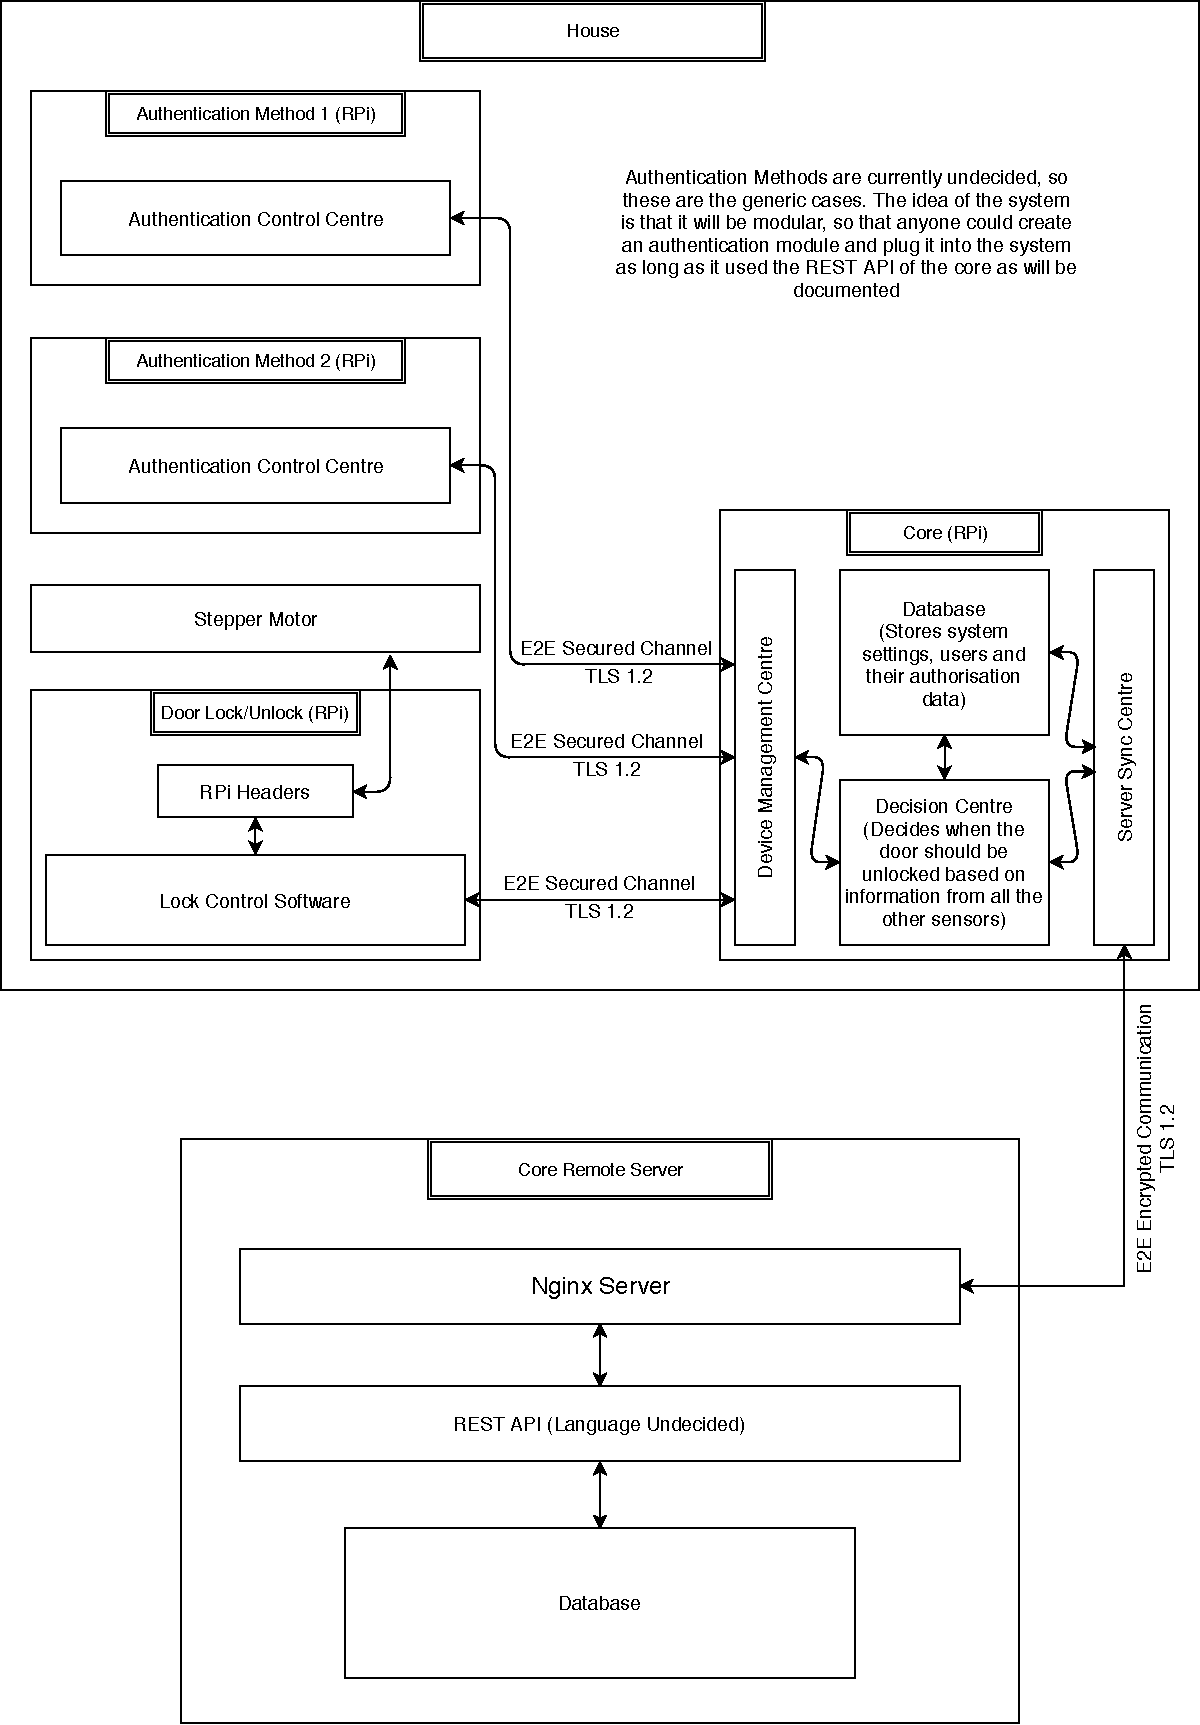
\includegraphics[height=0.6\textheight,keepaspectratio]{Graphics/FYP-Block-Diagram-Portrait}
\end{figure}

\subsection{Initial Core Raspberry Pi Setup}
Figure 4.2 below shows the planned sequence of interactions between different devices for setting up a new core raspberry pi including connecting it to the wifi and adding it to the users account. The initial setup section is mandatory, the alt section which allows the user to pair the device again at a later date is an optional implementation step and will be done if time permits.
\begin{figure}[H]
	\caption{Sequence Diagram for Setup of Core Raspberry Pi}
	\centering
		\includegraphics[height=0.6\textheight,keepaspectratio]{"Graphics/Initial Core RPi Setup"}
\end{figure}

\subsection{New Device Pairing to Existing Network}
Figure 4.3 below shows the planned sequence of interactions between different devices for setting up a new device when an existing network already exists, where a core has already been paired to an account. This process would add the new device to the existing core however this won't be needed if extra authentication methods aren't added to the network, again this will be time dependent.
\begin{figure}[H]
	\caption{Sequence Diagram for Setup of a New Device on an Existing Smart Lock Network}
	\centering
		\includegraphics[height=0.6\textheight,keepaspectratio]{"Graphics/New Device Pairing to Network"}
\end{figure}

\subsection{Technical Design Decisions}
In this section I will describe certain aspects of the project where I had to make decisions as to how they could be implemented best. In each section I will give a high level description of each method followed by which method I decided to go with and why. Some of the solutions may not be required as they may not get implemented in the demo, however they would be required for a full implementation and so are worth discussing.

\subsubsection*{Initiate Connection from Another Device to Core Raspberry Pi}
This is a difficult issue to get around as finding a specific device on the network is not trivial, especially if the network is particularly large. There are various different ways I could solve this which are described below.

\paragraph*{Method 1 - IP Broadcasting} One option is to use IP Broadcasting, where the core uses the networks broadcast range to send data to all the other devices on the network. This would work, but I'm unsure of the reliability of this method and broadcasting the IP of the core to the entire network doesn't seem like something I would want to do. It would likely be fine on a home network, however if it was on a much larger network in a business, this method may not work at all as they could block broadcasting on their switches entirely, or if multiple cores are running on the network it could become quite congested with the number of devices trying to announce themselves to other devices.

\paragraph*{Method 2 - Bluetooth Sync Device to Core} This would use the Bluetooth on both devices to contact each other and find out the IP of the core on the network. The device would then use this IP to establish a connection to the core. This method has a few issues, namely the security of communicating over Bluetooth as it doesn't have the same kind of security as Wi-Fi. The other issue is that this means the two devices must be within Bluetooth range, which is much shorter than Wi-Fi range and can't be easily extended, unlike Wi-Fi range which has highly available and cheap range extenders.

\paragraph*{Method 3 - Contact the remote server to get the Core IP} For this to work, the Core would have to announce its IP to the remote server whenever it changed. This would be very simple as the Core will already have a connection established to the remote server. The device that is trying to connect to the Core would then simply have to contact the remote server and request the IP of the Core on the local network, and then establish a connection with it. This is the easiest method to secure as it gives one point of contact to retrieve this information, and eliminates the need for any kind of discovery. This also allows devices to be as far away from each other as required if they are on the same network.

\paragraph*{Decision}
Method 3 would be the best way to go about this as it provides the most security and is also the most simple to implement. Devices can quickly look up the IP whenever they need and have to be authorised in order to do so.

\subsubsection*{Initiate Connection to Core Raspberry Pi for Initial Setup}

\paragraph*{Method 1 – Connect using 4-digit code through the remote server}
The first issue here is that using a code means that you don’t have to be within proximity of the device to attach to it as it goes through the remote server to establish the link. There are some potential ways that attackers could guess or work out the code and then connect to it themselves, or find some way to force the remote server to override the owner of that Core. The initial setup should be handled on the Core itself, and the phone should not contact the remote server regarding this, the Core should contact the remote server to establish that a link has been created.

\paragraph*{Method 2 – Connect using Bluetooth sync between the Core and users phone}
This method requires that the user is close to the Core to establish a link with it as they must be within Bluetooth range and push a physical button on the device to start the pairing process. If the device is already paired to an account, then it will either need to be confirmed by the current account that they want to pair to a new account or they will need to wait for a timeout to expire before the pairing can be done (unless it is cancelled from the current owners account). Within the app, they will need to select the option to connect to a new Core, and then select the Core they want to pair with from the list. The phone will then establish a Bluetooth connection with the Core, the Core will generate a private key to identify itself, and will upload the public key to the remote server for validation when communicating with it. This will bind the Core to the account the user was logged into and they will then be able to add new devices and users to the Core, as well as modify the settings for the Core, all from the app.

\paragraph*{Method 3 – Connect to Wi-Fi network broadcasted by the Core on users phone}
This method requires that the used must be close to the Core to push the physical button on the device to create the Wi-Fi network to start the setup of the device. All other steps are the same as Method 2, however this method has the benefit of not requiring every device to have Bluetooth as well as Wi-Fi, lowering the physical size, cost and power required to run each device. Wi-Fi can also be more easily secured than Bluetooth, and I will carry out testing to see if I can lower the power of the Wi-Fi adapter when in access point mode to lower the range of the network, so the user must be close to the device when performing the initial setup.

\paragraph*{Decision}
Method 3 is the best way to do this as we are already using Wi-Fi so don't require extra hardware on the device, also interfacing with and securing Wi-Fi is easier than Bluetooth which will save time in the development stage. 

\subsubsection*{Initiate Connection from New Device to Core Raspberry Pi for Setup}

\paragraph*{Method 1 – Bluetooth pairing between Device and Core}
This method would work, but could introduce difficulties for the user as it requires the two devices to be close to each other as they must be within Bluetooth range. It would also require the core to store the Wi-Fi password in a readable form to give it to new devices that will also need it. This is not something that I want to do as that means if someone can access the device then they can access the Wi-Fi password and therefore the entire network.

\paragraph*{Method 2 – Bluetooth pairing between device and users phone}
This method will work in the same way as the initial setup of the core. The User will press a pairing button on the device itself, then go to an add device page on their phone (only available for people who are already admins of a Core). On this page they will see any devices that are in pairing mode that they can add to their network. Once they have added the device, the app will request they connect it to the same Wi-Fi network as the Core, and request the password for the network. The device will then have successfully been added to the door unlocking system, will exit syncing mode, and will then communicate with the Core directly. The user will see the device in their list of devices on their door unlocking system, and will be able to change any settings it has.

\paragraph*{Method 3 – Wi-Fi pairing between the device and users phone}
This method will work in the same way as method 2, however it will use Wi-Fi instead of Bluetooth for the setup, for the same reasons mentioned in Method 3 of the Initiate Connection to Core Raspberry Pi for Initial Setup section.

\paragraph*{Decision}
Method 3 has been chosen for the same reason as in the Initiate Connection to Core Raspberry Pi for Initial Setup section.

\section{Tools Used}

\subsection{Version Control}
Version control is a very useful tool that is used throughout the software engineering industry as it allows much better management of source code and development in general. It contains a complete history of all changes that have been made to the project from the very beginning. This is very useful if you need to revert a change or diagnose a problem and find what change may have caused it.
\\
\indent There are a wide range of different Version Control Software's (VCS), however I decided to go with Git. Git is a very extensive and powerful tool, and is by far the most widely used VCS out there. Git can run locally and remotely so you can push your changes to a remote server so that others can see them and they are backed up. I use the open source free software Gitlab in order to host my own Git server so I used this for all my Git projects.
\\
\indent Alongside git itself I used the WebStorm and Android Studio git integration to help with committing code and pushing it to the remote server as both of those IDEs come with git integration built in. I also worked with git on the command line for pulling down the code on the devices that were running it.

\subsection{Integrated Development Environments (IDEs)}
IDEs are extremely useful tools that come bundled with a huge array of features all aiming to make developing easier and less error prone. They offer features such as auto-completion, auto-generation of certain code snippets, detection of potential errors, git integration, and much more.

\subsubsection*{WebStorm}
One of the IDEs used widely in this project was WebStorm as all of the APIs were written in Node.js which WebStorm has support for. Built-in support for Node.js, npm, git and more made the development process much smoother and faster. WebStorm is part of a much larger suite of IDEs made by JetBrains, they also make IntelliJ which is what AndroidStudio is based off of.

\subsubsection*{Android Studio}
Android Studio is the other IDE that I used in this project as it basically required if you want to write applications for Android. It comes with all the tools you need to compile and run android apps, including virtual android devices, a package manager for different versions of the android api, and many other great and useful tools. Installing and running all of this manually would take a huge amount of time, so using this tool vastly decreases the amount of time required for development and testing iterations.

% Development and Implementation

% !TeX root = ../../main.tex
\chapter{Implementation}
\label{chap:implementation}
In this chapter I will give details of the implementation of the previously mentioned ideas and requirements. This will cover technical aspects of the implementation, problems experienced along the way, any tools used to aid development and discussion on what languages where used and why. This chapter will be split up into sections for each component of the system in order to discuss why certain choices were made for that specific platform.

\section{Tools Used}
\subsection{Version Control}
Version control is a very useful tool that is used throughout the software engineering industry as it allows much better management of source code and development in general. It contains a complete history of all changes that have been made to the project from the very beginning. This is very useful if you need to revert a change or diagnose a problem and find what change may have caused it.
\\
\indent There are a wide range of different Version Control Software's (VCS), however I decided to go with Git. Git is a very extensive and powerful tool, and is by far the most widely used VCS out there. Git can run locally and remotely so you can push your changes to a remote server so that others can see them and they are backed up. I use the open source free software Gitlab in order to host my own Git server so I used this for all my Git projects.
\\
\indent Alongside git itself I used the WebStorm and Android Studio git integration to help with committing code and pushing it to the remote server as both of those IDEs come with git integration built in. I also worked with git on the command line for pulling down the code on the devices that were running it.

\subsection{Integrated Development Environments (IDEs)}
IDEs are extremely useful tools that come bundled with a huge array of features all aiming to make developing easier and less error prone. They offer features such as auto-completion, auto-generation of certain code snippets, detection of potential errors, git integration, and much more.

\subsubsection*{WebStorm}
One of the IDEs used widely in this project was WebStorm as all of the APIs were written in Node.js which WebStorm has support for. Built-in support for Node.js, npm, git and more made the development process much smoother and faster. WebStorm is part of a much larger suite of IDEs made by JetBrains, they also make IntelliJ which is what AndroidStudio is based off of.

\subsubsection*{Android Studio}
Android Studio is the other IDE that I used in this project as it basically required if you want to write applications for Android. It comes with all the tools you need to compile and run android apps, including virtual android devices, a package manager for different versions of the android api, and many other great and useful tools. Installing and running all of this manually would take a huge amount of time, so using this tool vastly decreases the amount of time required for development and testing iterations.

\section{Central Server}
The first section of the project that I worked on was the central server. The reason for this was that every other part of the system would rely on this in some way, and so it would get in the way if not done early on in the project. The plan was that in the eyes of the other parts of the application, the central server would just be a REST API that they could call to send and retrieve data, and that data would get passed to the other parts of the application that required them.

\subsection{Programming Language}
For this section of the project I decided to go with Node.js as I have used it before to make REST APIs and it provides high performance and is very quick to develop in. I used it along with an API design tool called Swagger which allows you to create a specification for your entire API, automatically generating documentation for it. It can also automatically generate boilerplate code for the server side and client side applications to make development much faster, it's a really useful tool. One of the major dependencies used within my development was mongoose which is a library that allows you to connect to a MongoDB database and make database calls in an asynchronous way with minimal code. Node.js has the benefit of encouraging you to write everything in an asynchronous manner, so almost everything uses callbacks rather than conventional nested statements. This has a huge performance benefit as the entire application runs on multiple threads rather than just a single thread.

\subsection{Login API}
This was the first part of the server that needed to be written, and security was vital. I was originally going to go with a traditional OAuth system but that seemed over complex for what was needed, so I decided to go with a JSON Web Token (JWT) system. JWT's are stored by the client and are sent along with every request. They contain data that both the client and the server can read, as well as an encrypted hash of that same data using a key that is stored on the server. This hash means that the client can't modify the data and then send it to the server as then the encrypted hash wouldn't match. 
\\
\indent For my system, I wanted it to be possible to later build in a system where the user could invalidate any device that is logged into their account, forcing that device to login again. This would be useful if the device was stolen and the user didn't want the thief to be able to also get into their house. In order to accommodate this in the future, I designed the JWTs so that they contain an ID which is stored in the database which then links that ID to a User object. If the JWT needs to be invalidated, simply delete the ID from the database and the device will no longer be able to authenticate and will be forced to login again, requiring the username and password for the account.
\\
\indent This system is used for both users and devices except that a device doesn't require a username and password. A device can register itself with the system and receives a JWT in return, it gives the server it's UUID and name during this process. Once the device is registered, a user can then register it to their account.

\subsection{Device and User API}
The device API includes the login api section for devices, but also includes the ability for the device to query information about itself so that it can be continually updating based on what the user does. This is how it responds to lock and unlock requests for example. The User API has the ability to set the device that is linked to their account using the UUID of the device, this then binds the device to their account, and the user can then send lock/unlock requests to the device through the API and get the device status using the user API.

\subsection{Other Software}
The system runs Nginx which is a web server software, the Node.js API runs its own web server on localhost which the Nginx server forwards traffic to using a reverse proxy system. Docker is another piece of software that is used for this part of the system, this is due to the hardware it's running on being used for multiple other systems as it is my own personal home server so this keeps it isolated from the rest of the system. As mentioned above MongoDB was used for the database software, I chose this as it is fast and reliable and i've used it before on previous projects with amazing results, so it was an easy choice for me when deciding on a database software to use.

\section{Smart Lock Core - Raspberry Pi}
The next step of the project was to work on the APIs, hardware and software setup for the raspberry pi that would be at the core of the network. This stage was probably the second largest sticking point for the project as it required a lot of experimentation with the hardware to get it working in the exact way I required. There were also technical issues along the way that hindered my progress which I will detail below.

\subsection{Programming Language}
As with the central server, this was mostly API based and therefore all the code was again written in Node.js using mongoose for and MongoDB for the database to store whatever the Core would need locally. I chose MongoDB in this instance as the initial implementation of the software wouldn't need a database necessarily as it would only be storing a small amount of data, however for some of the optional requirements data would need to be stored locally and therefore it was better to set this up now rather than have to change everything later.

\subsection{Setting up a Wi-Fi Hotspot}
For this I decided to use the built-in Wi-Fi of the Raspberry Pi 3 (RPi) as it had the most information readily available about how to set it up to do this. This part required three pieces of software: dhcpcd; dnsmasq; and hostapd. The job of dhcpcd was to assign the Wi-Fi hardware an IP when the hotspot was brought online so that other devices could contact it once they connected to the Wi-Fi. Dnsmasq provided dhcp for the Wi-Fi hotspot itself so that people who connected to the Wi-Fi could get an IP so the RPi could respond to them. Finally hostapd was the piece of software that provided the hotspot itself, booting up the onboard Wi-Fi and broadcasting the network so that others could connect. These pieces of software worked together flawlessly, however the initial RPi that I was using had an issue with the built-in antenna so I spent a fair few hours trying to figure out why the range was only a couple of centimetres from the device which turned out to just be wasted time as a new RPi fixed the problem with the exact same setup. Once this was working, turning the Wi-Fi on and off required just two commands, which were controlled by the Node.js API whilst setup was in progress.

\subsection{Setup API}
The setup API is just a REST API in the same way that the core server is, however it only works on the IP of the Wi-Fi hotspot (192.168.4.1). This IP would be the same on every device so that the users phone knows what IP to use in order to access the setup API. The API has two endpoints, one which accepts the Wi-Fi details so it can connect to your home Wi-Fi and returns the UUID of the device, and another which tells you the status of the setup, either waiting, testing, failed, or completed. Once the status endpoint is called and returns completed, it waits 5 seconds and then shuts down the hotspot as the device is now successfully setup. The details endpoint however is a lot more complex, as after it has received the details from the user it does a lot of tasks in order to connect to the Wi-Fi network provided, check that it connects successfully, generate a new UUID for itself, send that to the central server to register the device and then respond to the users device with the new UUID it generated. The main issue I came up against with this system was having the Wi-Fi devices switch between hotspot mode and connecting to the access point automatically, as it would kick the users device off of the hotspot and cause issues. Instead of this I decided to add a second Wi-Fi adapter to the device via USB as it eased the complexity of this section slightly and reduced the likelihood of issues arising down the line.

\subsection{Core to Central Server Communication}
The core is constantly polling the server for any commands that it may receive. Originally I was planning to have a constantly open connection in the form of a websocket, however this uses more resources constantly on the server side and is less secure if somehow the TLS encryption of one session was cracked by an attacker. With new sessions, new nonces and encryption keys are generated and so even with the information from the last session, this new sessions security would not be lessened by the fact that the last session was decrypted. That said, the chances of a session getting decrypted are essentially impossible with current technology, so this is being overly secure if anything.

\section{Android Application}
The final section of this project is the Android App which is the only part that the user will see directly. Not being a creative type myself meant that creating the user interface for this app was fairly difficult as it needed to be easy to use and clear. I feel like i've done a good job with it overall and the setup process seems simple to me.

\subsection{Programming Language}
The Android Application was programmed in Java as that's the main language used for Android development and it's one I am very familiar with. I used a few dependencies to aid my development process, mostly in regard to making network requests. Retrofit is a library that provides a very simple way to turn a HTTP API into a Java interface, making network requests much simpler and cleaner to look at. RxJava is another dependency that I used as it works with Retrofit to make all of the network calls work in the background and fire callbacks when a response is received. With Android, working Asynchronously is very important as if you do requests on the UI thread, the entire interface will freeze which makes for a very bad user experience.

\subsection{Development}
The first section I worked on was the login and sign up screens, ensuring that they would appear as soon as the user opens the application for the first time. I went with a minimal approach, only asking for the information that is required and made moving between the signup and login screens just a single tap or swipe away. The next part I worked on was the device setup screen which is by far the most complex part of the app. This page alone requires controlling what Wi-Fi the device is connected to, making API calls to the core raspberry pi and the central server and waiting until the right time to move on to the next screen. This screen gave me a lot of problems due to the complexity of changing Wi-Fi networks whilst trying to make requests to different APIs. The final screen that I worked on was the home screen which allows you to lock or unlock the smart lock. Originally there was planned to be a little more functionality but due to time constraints I had to build a working demo and cut the more fancy features that I had planned.

\section{Improvements}
Here I will list any improvements I would make if I were to approach this project again with this experience in mind. I've learnt a lot from this project and there are certain things that I would change to make the project work better or improve overall security of the product.

\subsection{Wi-Fi Hotspot Security}
Whilst programming the Wi-Fi hotspot section of the android application, I realised that there was no possible way to verify that the device I was connecting to was the device that I had in front of me using the current hardware I had. By the time I realised this I wouldn't have had time to order the extra parts required to get it ready in time for a demo, however I came up with a solution to the problem. The issue lies within how certificate trust works, with a certificate authority validating that you own a domain and then providing a public and private key pair to you. In a private network like the one created with a hotspot, this is not possible, and creating your own self-signed certificate means that the android application can't verify which device it is connected to. This would allow someone who was waiting for you to setup your device to create another Wi-Fi hotspot with the same name and have you connect to them. By doing this they could get access to your Wi-Fi password as you wouldn't realise it wasn't the same device that you see in front of you. In order for the user to confirm this, I would want to add a small screen to the device that could display a short code or QR code that the phone could scan as this direct method of communication can be verified. The code would be a hash of the https certificates public key and so could be verified by the phone to ensure they match, and if they do you're connected to the right device. This is a very unlikely scenario anyway as it requires an attacker to be waiting outside your home for you to setup the smartlock, and realistically they have a very small window to mimic the smart lock Wi-Fi and have the user connect to them instead.

\subsection{Another Improvement}
\improvement{Write another improvement}

\section{Compared to other locks}
Based on the issues I mentioned with other known locks in my problem statement, I will now evaluate what I have done to remove those security risks in my smart lock.

\subsection{August Firmware Key}
This problem can't happen on my system due to the fact that no master key exists. Everything is based around the user accounts themselves and communication with the central server meaning you have to be able to authenticate with the server to unlock the smart lock. On top of that, every time the smart lock is setup, it generates a new UUID which is used to identify itself on the server, so there is no chance that another user could register the lock to their account in the few second window where the lock is unregistered to an account on the central server.

\subsection{Removing Users whilst Offline}
With the currently developed system, the lock doesn't operate when offline as that functionality wasn't implemented. However, with the plan for offline functionality that I outlined in the design section, this lock would not be vulnerable to this attack as specific offline keys would have to be distributed by the lock owner, or another person who was trusted with the responsibility to distribute offline keys. Once the system comes back online then the keys immediately stop working and the lock must then be operated using the normal user authentication methods. In the case of other locks, communication with the internet could be blocked to the smartlock and then an attacker could use a compromised device to access the lock as the lock owner would be unable to remove the compromised device from the lock without being at home.

% Development


% System Testing


% Conclusion
% !TeX root = ../../main.tex
%The conclusion is a key part of the dissertation. It should be the natural end-point of
%the flow of argument that started from the Introduction with the identification of the
%problem to be tackled. It should draw upon the problem description and the literature
%survey, using the results to compare the work done with the expected outcome and
%with previous or related work. It should draw together the lessons learnt from your
%critical evaluation of the development/ implementation/ research processes used within
%the project. It should lead to a set of natural conclusions about the achievements made
%and the ways in which the difficulties encountered would be tackled if the project were
%to be run again. It should clearly identify any contributions to current knowledge or
%practice that the project provides. The conclusion should therefore be the culmination
%of the project, highlighting the achievements of the project, identifying things that have
%been done well, noting areas which could have been done better or tackled in a different
%way, and relating the work of the project to your intended system (as detailed in the
%Introduction) and related work (as discussed in the Literature Survey).
\chapter{Conclusion}
\label{chap:conclusion}

% Include a Chapter names References to the table of content
\addcontentsline{toc}{chapter}{References}
% Rename Bibliography to References
\renewcommand\bibname{References}
\bibliography{references}

% Include list of all To-Do's
\listoftodos[Notes]

% Include authors publications and appendix section
% Appedix
\appendix

\begingroup

\chapter{Appendix Chapter}
\label{app:appendix_chapter}

\section{Appending Section}
\label{app:sec:appendix_section}
Include appendix items in either sections of chapters

\endgroup
\end{document}